\documentclass[tikz,border=0.5cm,12pt]{standalone}
\usepackage[fontsize=16pt]{fontsize}
\usepackage{util}
\usetikzlibrary{shapes.multipart}
\usetikzlibrary{decorations.pathreplacing,calligraphy}

\begin{document}
  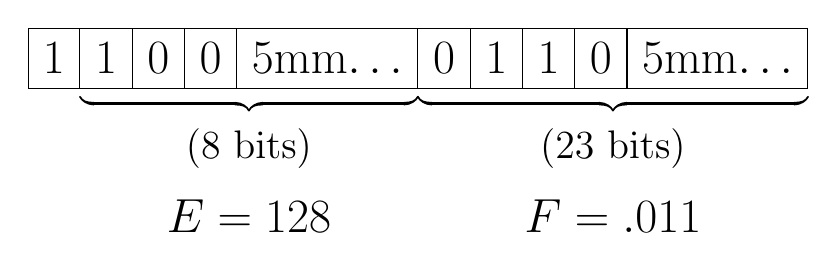
\begin{tikzpicture}[boxes/.style={
    rectangle split, rectangle split parts=#1, draw, anchor=center},
    curlybrace/.style={decoration={calligraphic brace, mirror, amplitude=5pt, raise=1mm}, decorate, line width=1.25pt}]
    \node [name=diagram, boxes=10, rectangle split horizontal] at (0, 0) {
      \nodepart{one} 1
      \nodepart{two} 1
      \nodepart{three} 0
      \nodepart{four} 0
      \nodepart{five} \pad{5mm}{$\dots$}
      \nodepart{six} 0
      \nodepart{seven} 1
      \nodepart{eight} 1
      \nodepart{nine} 0
      \nodepart{ten} \pad{5mm}{$\dots$}
    };

    \draw[curlybrace]
      (diagram.one split south) -- (diagram.five split south)
      node[midway, below=3mm] {\small (8 bits)}
      node[midway, below=12mm] {$E = 128$};
    \draw[curlybrace]
      (diagram.five split south) -- (diagram.south east)
      node[midway, below=3mm] {\small (23 bits)}
      node[midway, below=12mm] {$F = .011$};
  \end{tikzpicture}
\end{document}
